\documentclass[twoside]{book}

% Packages required by doxygen
\usepackage{fixltx2e}
\usepackage{calc}
\usepackage{doxygen}
\usepackage[export]{adjustbox} % also loads graphicx
\usepackage{graphicx}
\usepackage[utf8]{inputenc}
\usepackage{makeidx}
\usepackage{multicol}
\usepackage{multirow}
\PassOptionsToPackage{warn}{textcomp}
\usepackage{textcomp}
\usepackage[nointegrals]{wasysym}
\usepackage[table]{xcolor}

% Font selection
\usepackage[T1]{fontenc}
\usepackage[scaled=.90]{helvet}
\usepackage{courier}
\usepackage{amssymb}
\usepackage{sectsty}
\renewcommand{\familydefault}{\sfdefault}
\allsectionsfont{%
  \fontseries{bc}\selectfont%
  \color{darkgray}%
}
\renewcommand{\DoxyLabelFont}{%
  \fontseries{bc}\selectfont%
  \color{darkgray}%
}
\newcommand{\+}{\discretionary{\mbox{\scriptsize$\hookleftarrow$}}{}{}}

% Page & text layout
\usepackage{geometry}
\geometry{%
  a4paper,%
  top=2.5cm,%
  bottom=2.5cm,%
  left=2.5cm,%
  right=2.5cm%
}
\tolerance=750
\hfuzz=15pt
\hbadness=750
\setlength{\emergencystretch}{15pt}
\setlength{\parindent}{0cm}
\setlength{\parskip}{3ex plus 2ex minus 2ex}
\makeatletter
\renewcommand{\paragraph}{%
  \@startsection{paragraph}{4}{0ex}{-1.0ex}{1.0ex}{%
    \normalfont\normalsize\bfseries\SS@parafont%
  }%
}
\renewcommand{\subparagraph}{%
  \@startsection{subparagraph}{5}{0ex}{-1.0ex}{1.0ex}{%
    \normalfont\normalsize\bfseries\SS@subparafont%
  }%
}
\makeatother

% Headers & footers
\usepackage{fancyhdr}
\pagestyle{fancyplain}
\fancyhead[LE]{\fancyplain{}{\bfseries\thepage}}
\fancyhead[CE]{\fancyplain{}{}}
\fancyhead[RE]{\fancyplain{}{\bfseries\leftmark}}
\fancyhead[LO]{\fancyplain{}{\bfseries\rightmark}}
\fancyhead[CO]{\fancyplain{}{}}
\fancyhead[RO]{\fancyplain{}{\bfseries\thepage}}
\fancyfoot[LE]{\fancyplain{}{}}
\fancyfoot[CE]{\fancyplain{}{}}
\fancyfoot[RE]{\fancyplain{}{\bfseries\scriptsize Generated by Doxygen }}
\fancyfoot[LO]{\fancyplain{}{\bfseries\scriptsize Generated by Doxygen }}
\fancyfoot[CO]{\fancyplain{}{}}
\fancyfoot[RO]{\fancyplain{}{}}
\renewcommand{\footrulewidth}{0.4pt}
\renewcommand{\chaptermark}[1]{%
  \markboth{#1}{}%
}
\renewcommand{\sectionmark}[1]{%
  \markright{\thesection\ #1}%
}

% Indices & bibliography
\usepackage{natbib}
\usepackage[titles]{tocloft}
\setcounter{tocdepth}{3}
\setcounter{secnumdepth}{5}
\makeindex

% Hyperlinks (required, but should be loaded last)
\usepackage{ifpdf}
\ifpdf
  \usepackage[pdftex,pagebackref=true]{hyperref}
\else
  \usepackage[ps2pdf,pagebackref=true]{hyperref}
\fi
\hypersetup{%
  colorlinks=true,%
  linkcolor=blue,%
  citecolor=blue,%
  unicode%
}

% Custom commands
\newcommand{\clearemptydoublepage}{%
  \newpage{\pagestyle{empty}\cleardoublepage}%
}

\usepackage{caption}
\captionsetup{labelsep=space,justification=centering,font={bf},singlelinecheck=off,skip=4pt,position=top}

%===== C O N T E N T S =====

\begin{document}

% Titlepage & ToC
\hypersetup{pageanchor=false,
             bookmarksnumbered=true,
             pdfencoding=unicode
            }
\pagenumbering{roman}
\begin{titlepage}
\vspace*{7cm}
\begin{center}%
{\Large Line Follower Turtle\+Bot }\\
\vspace*{1cm}
{\large Generated by Doxygen 1.8.11}\\
\end{center}
\end{titlepage}
\clearemptydoublepage
\tableofcontents
\clearemptydoublepage
\pagenumbering{arabic}
\hypersetup{pageanchor=true}

%--- Begin generated contents ---
\chapter{Class Index}
\section{Class List}
Here are the classes, structs, unions and interfaces with brief descriptions\+:\begin{DoxyCompactList}
\item\contentsline{section}{\hyperlink{classLineDetect}{Line\+Detect} \\*Line Detect class contains all the functions for image procesing and direction publishing }{\pageref{classLineDetect}}{}
\item\contentsline{section}{\hyperlink{classturtlebot}{turtlebot} \\*Class turtlebot subscribes to the directions published and publishes velocity commands }{\pageref{classturtlebot}}{}
\end{DoxyCompactList}

\chapter{File Index}
\section{File List}
Here is a list of all documented files with brief descriptions\+:\begin{DoxyCompactList}
\item\contentsline{section}{/home/sudartion/catkin\+\_\+ws/src/line\+\_\+follower\+\_\+turtlebot/include/\hyperlink{linedetect_8hpp}{linedetect.\+hpp} \\*Header file for class linedetect }{\pageref{linedetect_8hpp}}{}
\item\contentsline{section}{/home/sudartion/catkin\+\_\+ws/src/line\+\_\+follower\+\_\+turtlebot/include/\hyperlink{turtlebot_8hpp}{turtlebot.\+hpp} \\*Class definition for turtlebot }{\pageref{turtlebot_8hpp}}{}
\item\contentsline{section}{/home/sudartion/catkin\+\_\+ws/src/line\+\_\+follower\+\_\+turtlebot/src/\hyperlink{detect_8cpp}{detect.\+cpp} \\*Ros Nod to subscribe to turtlebot images and perform image processing to detect line }{\pageref{detect_8cpp}}{}
\item\contentsline{section}{/home/sudartion/catkin\+\_\+ws/src/line\+\_\+follower\+\_\+turtlebot/src/\hyperlink{linedetect_8cpp}{linedetect.\+cpp} \\*Class linedetect\textquotesingle{}s function definitions }{\pageref{linedetect_8cpp}}{}
\item\contentsline{section}{/home/sudartion/catkin\+\_\+ws/src/line\+\_\+follower\+\_\+turtlebot/src/\hyperlink{motion__node_8cpp}{motion\+\_\+node.\+cpp} \\*Ros node to read direction to move in and publish velocity to turtlebot }{\pageref{motion__node_8cpp}}{}
\item\contentsline{section}{/home/sudartion/catkin\+\_\+ws/src/line\+\_\+follower\+\_\+turtlebot/src/\hyperlink{turtlebot_8cpp}{turtlebot.\+cpp} \\*Functions definitions for turtlebot class }{\pageref{turtlebot_8cpp}}{}
\item\contentsline{section}{/home/sudartion/catkin\+\_\+ws/src/line\+\_\+follower\+\_\+turtlebot/test/\hyperlink{test__detect_8cpp}{test\+\_\+detect.\+cpp} \\*Unit Test for all the functions in the detection class }{\pageref{test__detect_8cpp}}{}
\item\contentsline{section}{/home/sudartion/catkin\+\_\+ws/src/line\+\_\+follower\+\_\+turtlebot/test/\hyperlink{test__navig_8cpp}{test\+\_\+navig.\+cpp} \\*Unit Test for all the functions in the turtlebot navigation class }{\pageref{test__navig_8cpp}}{}
\end{DoxyCompactList}

\chapter{Class Documentation}
\hypertarget{classLineDetect}{}\section{Line\+Detect Class Reference}
\label{classLineDetect}\index{Line\+Detect@{Line\+Detect}}


Line Detect class contains all the functions for image procesing and direction publishing.  




{\ttfamily \#include $<$linedetect.\+hpp$>$}

\subsection*{Public Member Functions}
\begin{DoxyCompactItemize}
\item 
void \hyperlink{classLineDetect_a55952d3dc713611f47293aa16d9d1459}{image\+Callback} (const sensor\+\_\+msgs\+::\+Image\+Const\+Ptr \&msg)
\begin{DoxyCompactList}\small\item\em Direction message to be published. \end{DoxyCompactList}\item 
cv\+::\+Mat \hyperlink{classLineDetect_a95f915b8096799a874d5cec002f3dca3}{Gauss} (cv\+::\+Mat input)
\begin{DoxyCompactList}\small\item\em Function that applies Gaussian filter in the input image. \end{DoxyCompactList}\item 
int \hyperlink{classLineDetect_a35170d9af8b1baab0587b87475c94634}{colorthresh} (cv\+::\+Mat input)
\begin{DoxyCompactList}\small\item\em Function to perform line detection using color thresholding,image masking and centroid detection to publish direction. \end{DoxyCompactList}\end{DoxyCompactItemize}
\subsection*{Public Attributes}
\begin{DoxyCompactItemize}
\item 
cv\+::\+Mat {\bfseries img}\hypertarget{classLineDetect_a3b07274ae56a9f967a7b65d9650a057b}{}\label{classLineDetect_a3b07274ae56a9f967a7b65d9650a057b}

\item 
cv\+::\+Mat \hyperlink{classLineDetect_a9f63814c1f656cab53bd339d1eab70bc}{img\+\_\+filt}\hypertarget{classLineDetect_a9f63814c1f656cab53bd339d1eab70bc}{}\label{classLineDetect_a9f63814c1f656cab53bd339d1eab70bc}

\begin{DoxyCompactList}\small\item\em Input image in opencv matrix format. \end{DoxyCompactList}\item 
int \hyperlink{classLineDetect_a4745d206a2038e40341112670d0052d6}{dir}\hypertarget{classLineDetect_a4745d206a2038e40341112670d0052d6}{}\label{classLineDetect_a4745d206a2038e40341112670d0052d6}

\begin{DoxyCompactList}\small\item\em Filtered image in opencv matrix format. \end{DoxyCompactList}\end{DoxyCompactItemize}


\subsection{Detailed Description}
Line Detect class contains all the functions for image procesing and direction publishing. 

\subsection{Member Function Documentation}
\index{Line\+Detect@{Line\+Detect}!colorthresh@{colorthresh}}
\index{colorthresh@{colorthresh}!Line\+Detect@{Line\+Detect}}
\subsubsection[{\texorpdfstring{colorthresh(cv\+::\+Mat input)}{colorthresh(cv::Mat input)}}]{\setlength{\rightskip}{0pt plus 5cm}int Line\+Detect\+::colorthresh (
\begin{DoxyParamCaption}
\item[{cv\+::\+Mat}]{input}
\end{DoxyParamCaption}
)}\hypertarget{classLineDetect_a35170d9af8b1baab0587b87475c94634}{}\label{classLineDetect_a35170d9af8b1baab0587b87475c94634}


Function to perform line detection using color thresholding,image masking and centroid detection to publish direction. 


\begin{DoxyParams}{Parameters}
{\em input} & is the Filtered input image in opencv matrix format \\
\hline
\end{DoxyParams}
\begin{DoxyReturn}{Returns}
int direction which returns the direction the turtlebot should head in 
\end{DoxyReturn}
\index{Line\+Detect@{Line\+Detect}!Gauss@{Gauss}}
\index{Gauss@{Gauss}!Line\+Detect@{Line\+Detect}}
\subsubsection[{\texorpdfstring{Gauss(cv\+::\+Mat input)}{Gauss(cv::Mat input)}}]{\setlength{\rightskip}{0pt plus 5cm}cv\+::\+Mat Line\+Detect\+::\+Gauss (
\begin{DoxyParamCaption}
\item[{cv\+::\+Mat}]{input}
\end{DoxyParamCaption}
)}\hypertarget{classLineDetect_a95f915b8096799a874d5cec002f3dca3}{}\label{classLineDetect_a95f915b8096799a874d5cec002f3dca3}


Function that applies Gaussian filter in the input image. 


\begin{DoxyParams}{Parameters}
{\em input} & is the image from the turtlebot in opencv matrix format \\
\hline
\end{DoxyParams}
\begin{DoxyReturn}{Returns}
Mat of Gaussian filtered image in opencv matrix format 
\end{DoxyReturn}
\index{Line\+Detect@{Line\+Detect}!image\+Callback@{image\+Callback}}
\index{image\+Callback@{image\+Callback}!Line\+Detect@{Line\+Detect}}
\subsubsection[{\texorpdfstring{image\+Callback(const sensor\+\_\+msgs\+::\+Image\+Const\+Ptr \&msg)}{imageCallback(const sensor_msgs::ImageConstPtr &msg)}}]{\setlength{\rightskip}{0pt plus 5cm}void Line\+Detect\+::image\+Callback (
\begin{DoxyParamCaption}
\item[{const sensor\+\_\+msgs\+::\+Image\+Const\+Ptr \&}]{msg}
\end{DoxyParamCaption}
)}\hypertarget{classLineDetect_a55952d3dc713611f47293aa16d9d1459}{}\label{classLineDetect_a55952d3dc713611f47293aa16d9d1459}


Direction message to be published. 

Callback used to subscribe to the image topic from the Turtlebot and convert to opencv image format 
\begin{DoxyParams}{Parameters}
{\em msg} & is the image message for R\+OS \\
\hline
\end{DoxyParams}
\begin{DoxyReturn}{Returns}
none 
\end{DoxyReturn}


The documentation for this class was generated from the following files\+:\begin{DoxyCompactItemize}
\item 
/home/sudartion/catkin\+\_\+ws/src/line\+\_\+follower\+\_\+turtlebot/include/\hyperlink{linedetect_8hpp}{linedetect.\+hpp}\item 
/home/sudartion/catkin\+\_\+ws/src/line\+\_\+follower\+\_\+turtlebot/src/\hyperlink{linedetect_8cpp}{linedetect.\+cpp}\end{DoxyCompactItemize}

\hypertarget{classturtlebot}{}\section{turtlebot Class Reference}
\label{classturtlebot}\index{turtlebot@{turtlebot}}


Class turtlebot subscribes to the directions published and publishes velocity commands.  




{\ttfamily \#include $<$turtlebot.\+hpp$>$}

\subsection*{Public Member Functions}
\begin{DoxyCompactItemize}
\item 
void \hyperlink{classturtlebot_a086689860adb5ae052b5b89b17a79b7d}{dir\+\_\+sub} (line\+\_\+follower\+\_\+turtlebot\+::pos msg)
\begin{DoxyCompactList}\small\item\em Callback used to subscribe to the direction message published by the Line detection node. \end{DoxyCompactList}\item 
void \hyperlink{classturtlebot_a644fb3325e04d96fe171f8a773eba6b4}{vel\+\_\+cmd} (geometry\+\_\+msgs\+::\+Twist \&velocity, ros\+::\+Publisher \&pub, ros\+::\+Rate \&rate)
\begin{DoxyCompactList}\small\item\em Function to publish velocity commands based on direction. \end{DoxyCompactList}\end{DoxyCompactItemize}
\subsection*{Public Attributes}
\begin{DoxyCompactItemize}
\item 
int {\bfseries dir}\hypertarget{classturtlebot_a1d9acb8a367d808a4d4c897deab8b20c}{}\label{classturtlebot_a1d9acb8a367d808a4d4c897deab8b20c}

\end{DoxyCompactItemize}


\subsection{Detailed Description}
Class turtlebot subscribes to the directions published and publishes velocity commands. 

\subsection{Member Function Documentation}
\index{turtlebot@{turtlebot}!dir\+\_\+sub@{dir\+\_\+sub}}
\index{dir\+\_\+sub@{dir\+\_\+sub}!turtlebot@{turtlebot}}
\subsubsection[{\texorpdfstring{dir\+\_\+sub(line\+\_\+follower\+\_\+turtlebot\+::pos msg)}{dir_sub(line_follower_turtlebot::pos msg)}}]{\setlength{\rightskip}{0pt plus 5cm}void turtlebot\+::dir\+\_\+sub (
\begin{DoxyParamCaption}
\item[{line\+\_\+follower\+\_\+turtlebot\+::pos}]{msg}
\end{DoxyParamCaption}
)}\hypertarget{classturtlebot_a086689860adb5ae052b5b89b17a79b7d}{}\label{classturtlebot_a086689860adb5ae052b5b89b17a79b7d}


Callback used to subscribe to the direction message published by the Line detection node. 


\begin{DoxyParams}{Parameters}
{\em msg} & is the custom message pos which publishes a direction int between 0 and 3 \\
\hline
\end{DoxyParams}
\begin{DoxyReturn}{Returns}
none 
\end{DoxyReturn}
\index{turtlebot@{turtlebot}!vel\+\_\+cmd@{vel\+\_\+cmd}}
\index{vel\+\_\+cmd@{vel\+\_\+cmd}!turtlebot@{turtlebot}}
\subsubsection[{\texorpdfstring{vel\+\_\+cmd(geometry\+\_\+msgs\+::\+Twist \&velocity, ros\+::\+Publisher \&pub, ros\+::\+Rate \&rate)}{vel_cmd(geometry_msgs::Twist &velocity, ros::Publisher &pub, ros::Rate &rate)}}]{\setlength{\rightskip}{0pt plus 5cm}void turtlebot\+::vel\+\_\+cmd (
\begin{DoxyParamCaption}
\item[{geometry\+\_\+msgs\+::\+Twist \&}]{velocity, }
\item[{ros\+::\+Publisher \&}]{pub, }
\item[{ros\+::\+Rate \&}]{rate}
\end{DoxyParamCaption}
)}\hypertarget{classturtlebot_a644fb3325e04d96fe171f8a773eba6b4}{}\label{classturtlebot_a644fb3325e04d96fe171f8a773eba6b4}


Function to publish velocity commands based on direction. 


\begin{DoxyParams}{Parameters}
{\em velocity} & is the twist \\
\hline
{\em pub} & is used to publish the velocity commands to the turtlebot \\
\hline
{\em rate} & is the ros loop rate for publishing the commands \\
\hline
\end{DoxyParams}
\begin{DoxyReturn}{Returns}
none 
\end{DoxyReturn}


The documentation for this class was generated from the following files\+:\begin{DoxyCompactItemize}
\item 
/home/sudartion/catkin\+\_\+ws/src/line\+\_\+follower\+\_\+turtlebot/include/\hyperlink{turtlebot_8hpp}{turtlebot.\+hpp}\item 
/home/sudartion/catkin\+\_\+ws/src/line\+\_\+follower\+\_\+turtlebot/src/\hyperlink{turtlebot_8cpp}{turtlebot.\+cpp}\end{DoxyCompactItemize}

\chapter{File Documentation}
\hypertarget{linedetect_8hpp}{}\section{/home/sudartion/catkin\+\_\+ws/src/line\+\_\+follower\+\_\+turtlebot/include/linedetect.hpp File Reference}
\label{linedetect_8hpp}\index{/home/sudartion/catkin\+\_\+ws/src/line\+\_\+follower\+\_\+turtlebot/include/linedetect.\+hpp@{/home/sudartion/catkin\+\_\+ws/src/line\+\_\+follower\+\_\+turtlebot/include/linedetect.\+hpp}}


Header file for class linedetect.  


{\ttfamily \#include $<$opencv2/highgui/highgui.\+hpp$>$}\\*
{\ttfamily \#include $<$cv\+\_\+bridge/cv\+\_\+bridge.\+h$>$}\\*
{\ttfamily \#include $<$vector$>$}\\*
{\ttfamily \#include \char`\"{}opencv2/opencv.\+hpp\char`\"{}}\\*
{\ttfamily \#include \char`\"{}ros/ros.\+h\char`\"{}}\\*
{\ttfamily \#include \char`\"{}line\+\_\+follower\+\_\+turtlebot/pos.\+h\char`\"{}}\\*
Include dependency graph for linedetect.\+hpp\+:\nopagebreak
\begin{figure}[H]
\begin{center}
\leavevmode
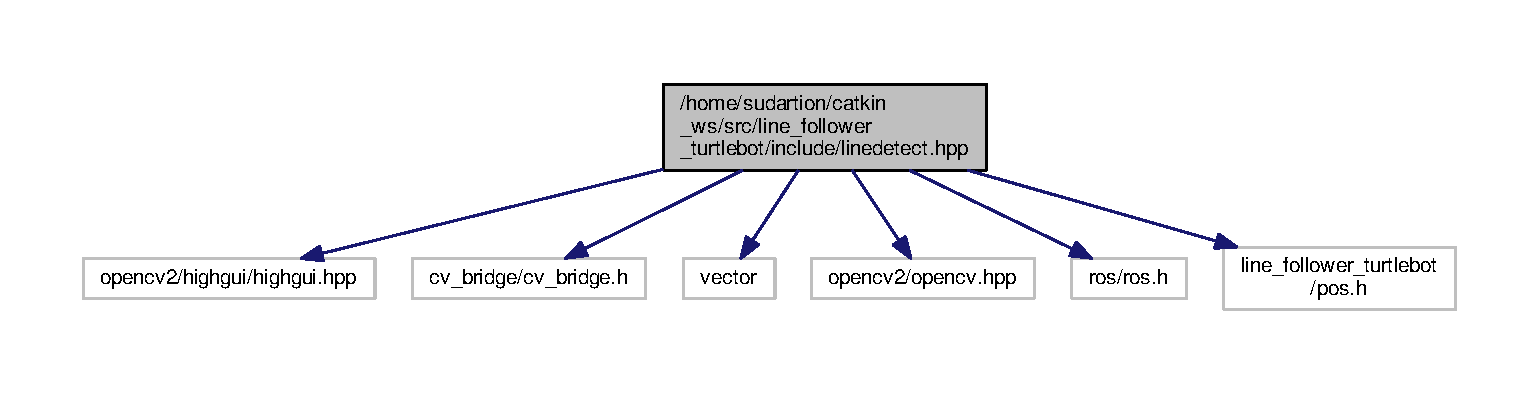
\includegraphics[width=350pt]{linedetect_8hpp__incl}
\end{center}
\end{figure}
This graph shows which files directly or indirectly include this file\+:\nopagebreak
\begin{figure}[H]
\begin{center}
\leavevmode
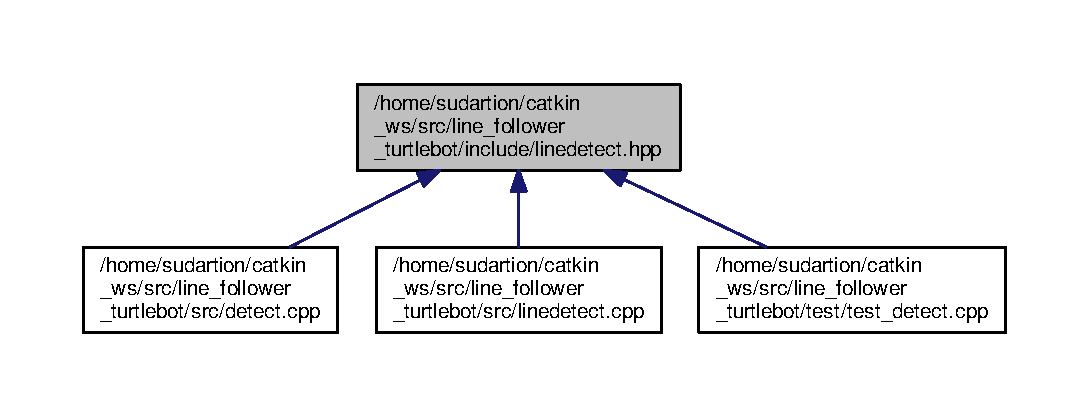
\includegraphics[width=350pt]{linedetect_8hpp__dep__incl}
\end{center}
\end{figure}
\subsection*{Classes}
\begin{DoxyCompactItemize}
\item 
class \hyperlink{classLineDetect}{Line\+Detect}
\begin{DoxyCompactList}\small\item\em Line Detect class contains all the functions for image procesing and direction publishing. \end{DoxyCompactList}\end{DoxyCompactItemize}


\subsection{Detailed Description}
Header file for class linedetect. 

M\+IT License Copyright (c) 2017 Sudarshan Raghunathan Permission is hereby granted, free of charge, to any person obtaining a copy of this software and associated documentation files (the \char`\"{}\+Software\char`\"{}), to deal in the Software without restriction, including without limitation the rights to use, copy, modify, merge, publish, distribute, sublicense, and/or sell copies of the Software, and to permit persons to whom the Software is furnished to do so, subject to the following conditions\+: The above copyright notice and this permission notice shall be included in all copies or substantial portions of the Software. T\+HE S\+O\+F\+T\+W\+A\+RE IS P\+R\+O\+V\+I\+D\+ED \char`\"{}\+A\+S I\+S\char`\"{}, W\+I\+T\+H\+O\+UT W\+A\+R\+R\+A\+N\+TY OF A\+NY K\+I\+ND, E\+X\+P\+R\+E\+SS OR I\+M\+P\+L\+I\+ED, I\+N\+C\+L\+U\+D\+I\+NG B\+UT N\+OT L\+I\+M\+I\+T\+ED TO T\+HE W\+A\+R\+R\+A\+N\+T\+I\+ES OF M\+E\+R\+C\+H\+A\+N\+T\+A\+B\+I\+L\+I\+TY, F\+I\+T\+N\+E\+SS F\+OR A P\+A\+R\+T\+I\+C\+U\+L\+AR P\+U\+R\+P\+O\+SE A\+ND N\+O\+N\+I\+N\+F\+R\+I\+N\+G\+E\+M\+E\+NT. IN NO E\+V\+E\+NT S\+H\+A\+LL T\+HE A\+U\+T\+H\+O\+RS OR C\+O\+P\+Y\+R\+I\+G\+HT H\+O\+L\+D\+E\+RS BE L\+I\+A\+B\+LE F\+OR A\+NY C\+L\+A\+IM, D\+A\+M\+A\+G\+ES OR O\+T\+H\+ER L\+I\+A\+B\+I\+L\+I\+TY, W\+H\+E\+T\+H\+ER IN AN A\+C\+T\+I\+ON OF C\+O\+N\+T\+R\+A\+CT, T\+O\+RT OR O\+T\+H\+E\+R\+W\+I\+SE, A\+R\+I\+S\+I\+NG F\+R\+OM, O\+UT OF OR IN C\+O\+N\+N\+E\+C\+T\+I\+ON W\+I\+TH T\+HE S\+O\+F\+T\+W\+A\+RE OR T\+HE U\+SE OR O\+T\+H\+ER D\+E\+A\+L\+I\+N\+GS IN T\+HE S\+O\+F\+T\+W\+A\+RE.

\begin{DoxyCopyright}{Copyright}
Copyright 2017 Sudarshan Raghunathan
\end{DoxyCopyright}
\begin{DoxyAuthor}{Author}
Sudarshan Raghunathan 
\end{DoxyAuthor}

\hypertarget{turtlebot_8hpp}{}\section{/home/sudartion/catkin\+\_\+ws/src/line\+\_\+follower\+\_\+turtlebot/include/turtlebot.hpp File Reference}
\label{turtlebot_8hpp}\index{/home/sudartion/catkin\+\_\+ws/src/line\+\_\+follower\+\_\+turtlebot/include/turtlebot.\+hpp@{/home/sudartion/catkin\+\_\+ws/src/line\+\_\+follower\+\_\+turtlebot/include/turtlebot.\+hpp}}


Class definition for turtlebot.  


{\ttfamily \#include $<$geometry\+\_\+msgs/\+Twist.\+h$>$}\\*
{\ttfamily \#include $<$vector$>$}\\*
{\ttfamily \#include \char`\"{}ros/ros.\+h\char`\"{}}\\*
{\ttfamily \#include \char`\"{}line\+\_\+follower\+\_\+turtlebot/pos.\+h\char`\"{}}\\*
Include dependency graph for turtlebot.\+hpp\+:\nopagebreak
\begin{figure}[H]
\begin{center}
\leavevmode
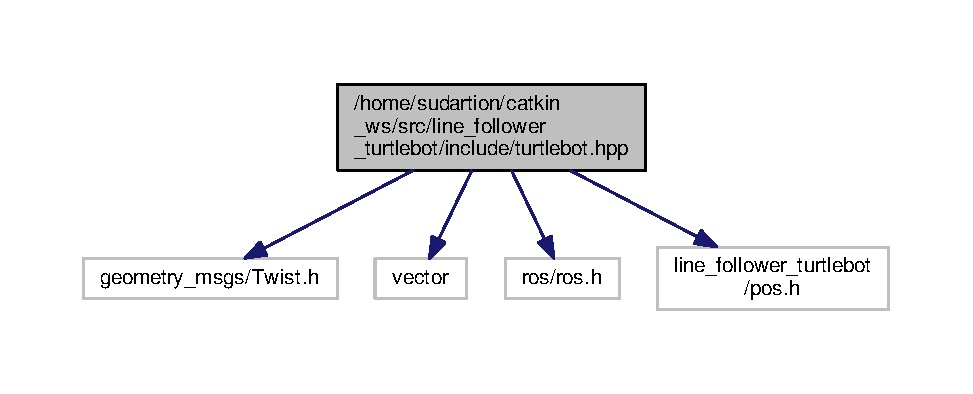
\includegraphics[width=350pt]{turtlebot_8hpp__incl}
\end{center}
\end{figure}
This graph shows which files directly or indirectly include this file\+:\nopagebreak
\begin{figure}[H]
\begin{center}
\leavevmode
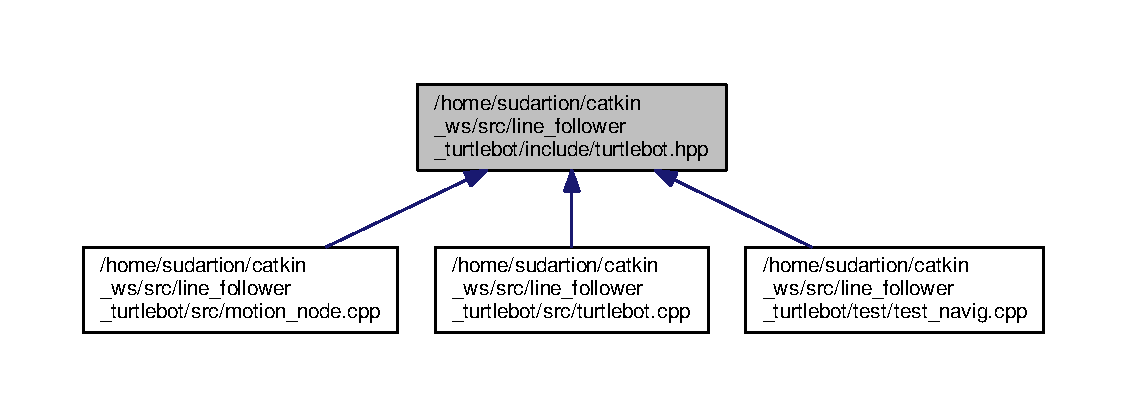
\includegraphics[width=350pt]{turtlebot_8hpp__dep__incl}
\end{center}
\end{figure}
\subsection*{Classes}
\begin{DoxyCompactItemize}
\item 
class \hyperlink{classturtlebot}{turtlebot}
\begin{DoxyCompactList}\small\item\em Class turtlebot subscribes to the directions published and publishes velocity commands. \end{DoxyCompactList}\end{DoxyCompactItemize}


\subsection{Detailed Description}
Class definition for turtlebot. 

M\+IT License Copyright (c) 2017 Sudarshan Raghunathan Permission is hereby granted, free of charge, to any person obtaining a copy of this software and associated documentation files (the \char`\"{}\+Software\char`\"{}), to deal in the Software without restriction, including without limitation the rights to use, copy, modify, merge, publish, distribute, sublicense, and/or sell copies of the Software, and to permit persons to whom the Software is furnished to do so, subject to the following conditions\+: The above copyright notice and this permission notice shall be included in all copies or substantial portions of the Software. T\+HE S\+O\+F\+T\+W\+A\+RE IS P\+R\+O\+V\+I\+D\+ED \char`\"{}\+A\+S I\+S\char`\"{}, W\+I\+T\+H\+O\+UT W\+A\+R\+R\+A\+N\+TY OF A\+NY K\+I\+ND, E\+X\+P\+R\+E\+SS OR I\+M\+P\+L\+I\+ED, I\+N\+C\+L\+U\+D\+I\+NG B\+UT N\+OT L\+I\+M\+I\+T\+ED TO T\+HE W\+A\+R\+R\+A\+N\+T\+I\+ES OF M\+E\+R\+C\+H\+A\+N\+T\+A\+B\+I\+L\+I\+TY, F\+I\+T\+N\+E\+SS F\+OR A P\+A\+R\+T\+I\+C\+U\+L\+AR P\+U\+R\+P\+O\+SE A\+ND N\+O\+N\+I\+N\+F\+R\+I\+N\+G\+E\+M\+E\+NT. IN NO E\+V\+E\+NT S\+H\+A\+LL T\+HE A\+U\+T\+H\+O\+RS OR C\+O\+P\+Y\+R\+I\+G\+HT H\+O\+L\+D\+E\+RS BE L\+I\+A\+B\+LE F\+OR A\+NY C\+L\+A\+IM, D\+A\+M\+A\+G\+ES OR O\+T\+H\+ER L\+I\+A\+B\+I\+L\+I\+TY, W\+H\+E\+T\+H\+ER IN AN A\+C\+T\+I\+ON OF C\+O\+N\+T\+R\+A\+CT, T\+O\+RT OR O\+T\+H\+E\+R\+W\+I\+SE, A\+R\+I\+S\+I\+NG F\+R\+OM, O\+UT OF OR IN C\+O\+N\+N\+E\+C\+T\+I\+ON W\+I\+TH T\+HE S\+O\+F\+T\+W\+A\+RE OR T\+HE U\+SE OR O\+T\+H\+ER D\+E\+A\+L\+I\+N\+GS IN T\+HE S\+O\+F\+T\+W\+A\+RE.

\begin{DoxyCopyright}{Copyright}
Copyright 2017 Sudarshan Raghunathan
\end{DoxyCopyright}
\begin{DoxyAuthor}{Author}
Sudarshan Raghunathan 
\end{DoxyAuthor}

\hypertarget{detect_8cpp}{}\section{/home/sudartion/catkin\+\_\+ws/src/line\+\_\+follower\+\_\+turtlebot/src/detect.cpp File Reference}
\label{detect_8cpp}\index{/home/sudartion/catkin\+\_\+ws/src/line\+\_\+follower\+\_\+turtlebot/src/detect.\+cpp@{/home/sudartion/catkin\+\_\+ws/src/line\+\_\+follower\+\_\+turtlebot/src/detect.\+cpp}}


Ros Nod to subscribe to turtlebot images and perform image processing to detect line.  


{\ttfamily \#include $<$cstdlib$>$}\\*
{\ttfamily \#include $<$string$>$}\\*
{\ttfamily \#include $<$opencv2/highgui/highgui.\+hpp$>$}\\*
{\ttfamily \#include $<$cv\+\_\+bridge/cv\+\_\+bridge.\+h$>$}\\*
{\ttfamily \#include \char`\"{}opencv2/opencv.\+hpp\char`\"{}}\\*
{\ttfamily \#include \char`\"{}ros/ros.\+h\char`\"{}}\\*
{\ttfamily \#include \char`\"{}ros/console.\+h\char`\"{}}\\*
{\ttfamily \#include \char`\"{}linedetect.\+hpp\char`\"{}}\\*
{\ttfamily \#include \char`\"{}line\+\_\+follower\+\_\+turtlebot/pos.\+h\char`\"{}}\\*
Include dependency graph for detect.\+cpp\+:\nopagebreak
\begin{figure}[H]
\begin{center}
\leavevmode
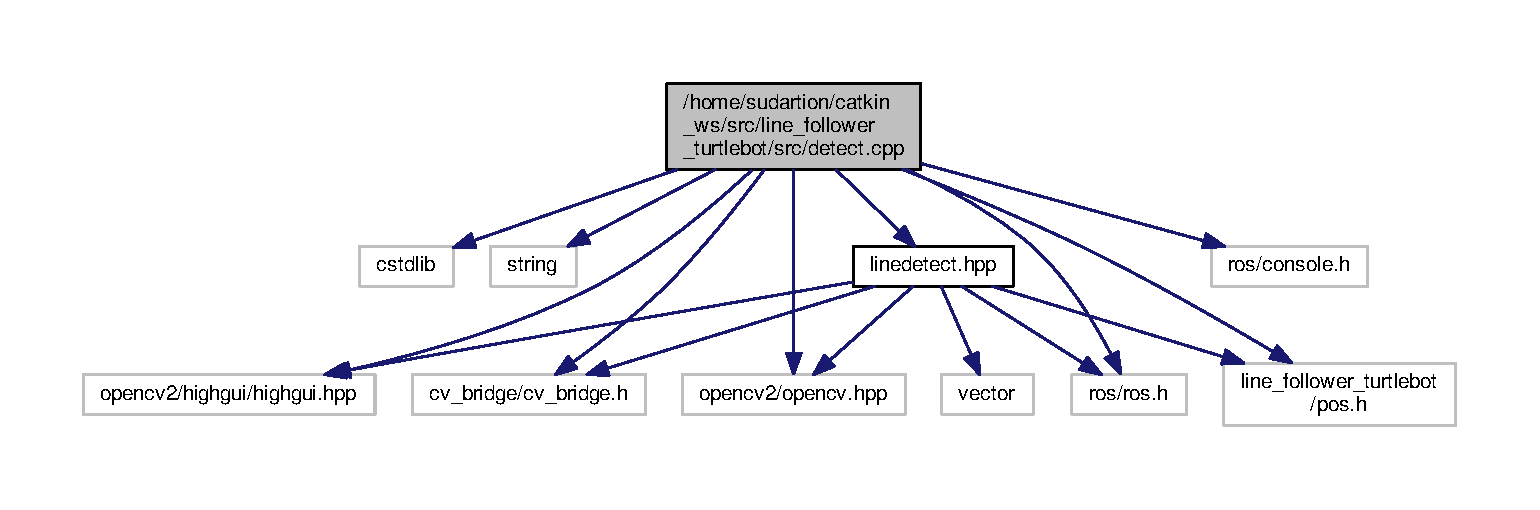
\includegraphics[width=350pt]{detect_8cpp__incl}
\end{center}
\end{figure}
\subsection*{Functions}
\begin{DoxyCompactItemize}
\item 
int \hyperlink{detect_8cpp_a3c04138a5bfe5d72780bb7e82a18e627}{main} (int argc, char $\ast$$\ast$argv)
\begin{DoxyCompactList}\small\item\em Main function that reads image from the turtlebot and provides direction to move using image processing. \end{DoxyCompactList}\end{DoxyCompactItemize}


\subsection{Detailed Description}
Ros Nod to subscribe to turtlebot images and perform image processing to detect line. 

M\+IT License Copyright (c) 2017 Sudarshan Raghunathan Permission is hereby granted, free of charge, to any person obtaining a copy of this software and associated documentation files (the \char`\"{}\+Software\char`\"{}), to deal in the Software without restriction, including without limitation the rights to use, copy, modify, merge, publish, distribute, sublicense, and/or sell copies of the Software, and to permit persons to whom the Software is furnished to do so, subject to the following conditions\+: The above copyright notice and this permission notice shall be included in all copies or substantial portions of the Software. T\+HE S\+O\+F\+T\+W\+A\+RE IS P\+R\+O\+V\+I\+D\+ED \char`\"{}\+A\+S I\+S\char`\"{}, W\+I\+T\+H\+O\+UT W\+A\+R\+R\+A\+N\+TY OF A\+NY K\+I\+ND, E\+X\+P\+R\+E\+SS OR I\+M\+P\+L\+I\+ED, I\+N\+C\+L\+U\+D\+I\+NG B\+UT N\+OT L\+I\+M\+I\+T\+ED TO T\+HE W\+A\+R\+R\+A\+N\+T\+I\+ES OF M\+E\+R\+C\+H\+A\+N\+T\+A\+B\+I\+L\+I\+TY, F\+I\+T\+N\+E\+SS F\+OR A P\+A\+R\+T\+I\+C\+U\+L\+AR P\+U\+R\+P\+O\+SE A\+ND N\+O\+N\+I\+N\+F\+R\+I\+N\+G\+E\+M\+E\+NT. IN NO E\+V\+E\+NT S\+H\+A\+LL T\+HE A\+U\+T\+H\+O\+RS OR C\+O\+P\+Y\+R\+I\+G\+HT H\+O\+L\+D\+E\+RS BE L\+I\+A\+B\+LE F\+OR A\+NY C\+L\+A\+IM, D\+A\+M\+A\+G\+ES OR O\+T\+H\+ER L\+I\+A\+B\+I\+L\+I\+TY, W\+H\+E\+T\+H\+ER IN AN A\+C\+T\+I\+ON OF C\+O\+N\+T\+R\+A\+CT, T\+O\+RT OR O\+T\+H\+E\+R\+W\+I\+SE, A\+R\+I\+S\+I\+NG F\+R\+OM, O\+UT OF OR IN C\+O\+N\+N\+E\+C\+T\+I\+ON W\+I\+TH T\+HE S\+O\+F\+T\+W\+A\+RE OR T\+HE U\+SE OR O\+T\+H\+ER D\+E\+A\+L\+I\+N\+GS IN T\+HE S\+O\+F\+T\+W\+A\+RE.

\begin{DoxyCopyright}{Copyright}
Copyright 2017 Sudarshan Raghunathan
\end{DoxyCopyright}
\begin{DoxyAuthor}{Author}
Sudarshan Raghunathan 
\end{DoxyAuthor}


\subsection{Function Documentation}
\index{detect.\+cpp@{detect.\+cpp}!main@{main}}
\index{main@{main}!detect.\+cpp@{detect.\+cpp}}
\subsubsection[{\texorpdfstring{main(int argc, char $\ast$$\ast$argv)}{main(int argc, char **argv)}}]{\setlength{\rightskip}{0pt plus 5cm}int main (
\begin{DoxyParamCaption}
\item[{int}]{argc, }
\item[{char $\ast$$\ast$}]{argv}
\end{DoxyParamCaption}
)}\hypertarget{detect_8cpp_a3c04138a5bfe5d72780bb7e82a18e627}{}\label{detect_8cpp_a3c04138a5bfe5d72780bb7e82a18e627}


Main function that reads image from the turtlebot and provides direction to move using image processing. 


\begin{DoxyParams}{Parameters}
{\em argc} & is the number of arguments of the main function \\
\hline
{\em argv} & is the array of arugments \\
\hline
\end{DoxyParams}
\begin{DoxyReturn}{Returns}
0 
\end{DoxyReturn}

\hypertarget{linedetect_8cpp}{}\section{/home/sudartion/catkin\+\_\+ws/src/line\+\_\+follower\+\_\+turtlebot/src/linedetect.cpp File Reference}
\label{linedetect_8cpp}\index{/home/sudartion/catkin\+\_\+ws/src/line\+\_\+follower\+\_\+turtlebot/src/linedetect.\+cpp@{/home/sudartion/catkin\+\_\+ws/src/line\+\_\+follower\+\_\+turtlebot/src/linedetect.\+cpp}}


Class linedetect\textquotesingle{}s function definitions.  


{\ttfamily \#include $<$cstdlib$>$}\\*
{\ttfamily \#include $<$string$>$}\\*
{\ttfamily \#include $<$opencv2/highgui/highgui.\+hpp$>$}\\*
{\ttfamily \#include $<$cv\+\_\+bridge/cv\+\_\+bridge.\+h$>$}\\*
{\ttfamily \#include \char`\"{}ros/ros.\+h\char`\"{}}\\*
{\ttfamily \#include \char`\"{}opencv2/opencv.\+hpp\char`\"{}}\\*
{\ttfamily \#include \char`\"{}ros/console.\+h\char`\"{}}\\*
{\ttfamily \#include \char`\"{}linedetect.\+hpp\char`\"{}}\\*
{\ttfamily \#include \char`\"{}line\+\_\+follower\+\_\+turtlebot/pos.\+h\char`\"{}}\\*
Include dependency graph for linedetect.\+cpp\+:\nopagebreak
\begin{figure}[H]
\begin{center}
\leavevmode
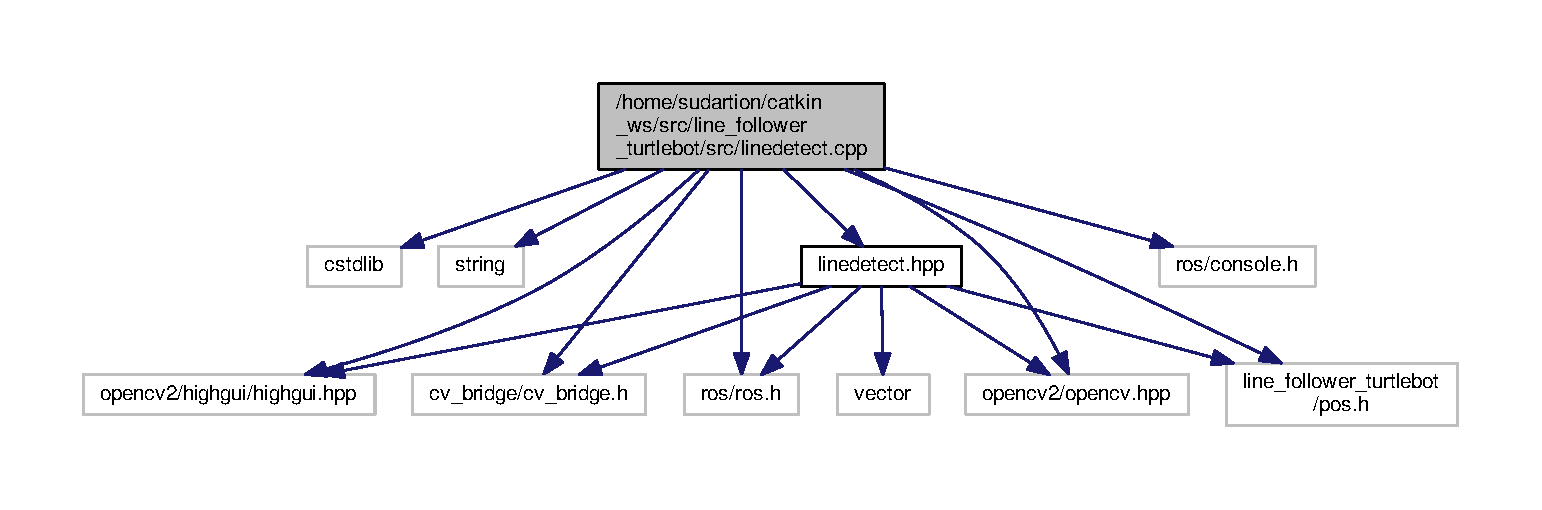
\includegraphics[width=350pt]{linedetect_8cpp__incl}
\end{center}
\end{figure}


\subsection{Detailed Description}
Class linedetect\textquotesingle{}s function definitions. 

M\+IT License Copyright (c) 2017 Sudarshan Raghunathan Permission is hereby granted, free of charge, to any person obtaining a copy of this software and associated documentation files (the \char`\"{}\+Software\char`\"{}), to deal in the Software without restriction, including without limitation the rights to use, copy, modify, merge, publish, distribute, sublicense, and/or sell copies of the Software, and to permit persons to whom the Software is furnished to do so, subject to the following conditions\+: The above copyright notice and this permission notice shall be included in all copies or substantial portions of the Software. T\+HE S\+O\+F\+T\+W\+A\+RE IS P\+R\+O\+V\+I\+D\+ED \char`\"{}\+A\+S I\+S\char`\"{}, W\+I\+T\+H\+O\+UT W\+A\+R\+R\+A\+N\+TY OF A\+NY K\+I\+ND, E\+X\+P\+R\+E\+SS OR I\+M\+P\+L\+I\+ED, I\+N\+C\+L\+U\+D\+I\+NG B\+UT N\+OT L\+I\+M\+I\+T\+ED TO T\+HE W\+A\+R\+R\+A\+N\+T\+I\+ES OF M\+E\+R\+C\+H\+A\+N\+T\+A\+B\+I\+L\+I\+TY, F\+I\+T\+N\+E\+SS F\+OR A P\+A\+R\+T\+I\+C\+U\+L\+AR P\+U\+R\+P\+O\+SE A\+ND N\+O\+N\+I\+N\+F\+R\+I\+N\+G\+E\+M\+E\+NT. IN NO E\+V\+E\+NT S\+H\+A\+LL T\+HE A\+U\+T\+H\+O\+RS OR C\+O\+P\+Y\+R\+I\+G\+HT H\+O\+L\+D\+E\+RS BE L\+I\+A\+B\+LE F\+OR A\+NY C\+L\+A\+IM, D\+A\+M\+A\+G\+ES OR O\+T\+H\+ER L\+I\+A\+B\+I\+L\+I\+TY, W\+H\+E\+T\+H\+ER IN AN A\+C\+T\+I\+ON OF C\+O\+N\+T\+R\+A\+CT, T\+O\+RT OR O\+T\+H\+E\+R\+W\+I\+SE, A\+R\+I\+S\+I\+NG F\+R\+OM, O\+UT OF OR IN C\+O\+N\+N\+E\+C\+T\+I\+ON W\+I\+TH T\+HE S\+O\+F\+T\+W\+A\+RE OR T\+HE U\+SE OR O\+T\+H\+ER D\+E\+A\+L\+I\+N\+GS IN T\+HE S\+O\+F\+T\+W\+A\+RE.

\begin{DoxyCopyright}{Copyright}
Copyright 2017 Sudarshan Raghunathan
\end{DoxyCopyright}
\begin{DoxyAuthor}{Author}
Sudarshan Raghunathan 
\end{DoxyAuthor}

\hypertarget{motion__node_8cpp}{}\section{/home/sudartion/catkin\+\_\+ws/src/line\+\_\+follower\+\_\+turtlebot/src/motion\+\_\+node.cpp File Reference}
\label{motion__node_8cpp}\index{/home/sudartion/catkin\+\_\+ws/src/line\+\_\+follower\+\_\+turtlebot/src/motion\+\_\+node.\+cpp@{/home/sudartion/catkin\+\_\+ws/src/line\+\_\+follower\+\_\+turtlebot/src/motion\+\_\+node.\+cpp}}


Ros node to read direction to move in and publish velocity to turtlebot.  


{\ttfamily \#include $<$cstdlib$>$}\\*
{\ttfamily \#include $<$string$>$}\\*
{\ttfamily \#include $<$opencv2/highgui/highgui.\+hpp$>$}\\*
{\ttfamily \#include $<$cv\+\_\+bridge/cv\+\_\+bridge.\+h$>$}\\*
{\ttfamily \#include \char`\"{}opencv2/opencv.\+hpp\char`\"{}}\\*
{\ttfamily \#include \char`\"{}ros/ros.\+h\char`\"{}}\\*
{\ttfamily \#include \char`\"{}ros/console.\+h\char`\"{}}\\*
{\ttfamily \#include \char`\"{}turtlebot.\+hpp\char`\"{}}\\*
{\ttfamily \#include \char`\"{}line\+\_\+follower\+\_\+turtlebot/pos.\+h\char`\"{}}\\*
Include dependency graph for motion\+\_\+node.\+cpp\+:\nopagebreak
\begin{figure}[H]
\begin{center}
\leavevmode
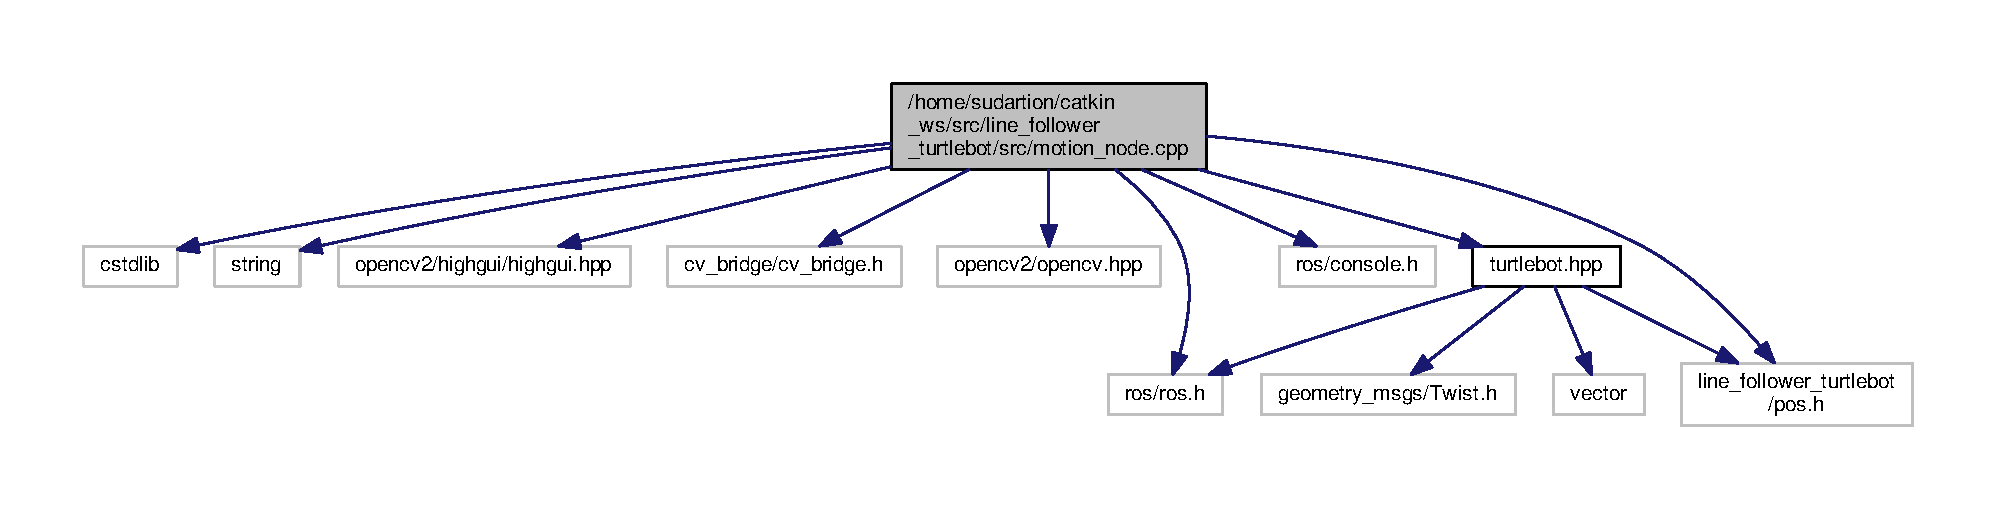
\includegraphics[width=350pt]{motion__node_8cpp__incl}
\end{center}
\end{figure}
\subsection*{Functions}
\begin{DoxyCompactItemize}
\item 
int \hyperlink{motion__node_8cpp_a3c04138a5bfe5d72780bb7e82a18e627}{main} (int argc, char $\ast$$\ast$argv)
\begin{DoxyCompactList}\small\item\em Main function that reads direction from the detect node and publishes velocity to the turtlebot at a given rate. \end{DoxyCompactList}\end{DoxyCompactItemize}


\subsection{Detailed Description}
Ros node to read direction to move in and publish velocity to turtlebot. 

M\+IT License Copyright (c) 2017 Sudarshan Raghunathan Permission is hereby granted, free of charge, to any person obtaining a copy of this software and associated documentation files (the \char`\"{}\+Software\char`\"{}), to deal in the Software without restriction, including without limitation the rights to use, copy, modify, merge, publish, distribute, sublicense, and/or sell copies of the Software, and to permit persons to whom the Software is furnished to do so, subject to the following conditions\+: The above copyright notice and this permission notice shall be included in all copies or substantial portions of the Software. T\+HE S\+O\+F\+T\+W\+A\+RE IS P\+R\+O\+V\+I\+D\+ED \char`\"{}\+A\+S I\+S\char`\"{}, W\+I\+T\+H\+O\+UT W\+A\+R\+R\+A\+N\+TY OF A\+NY K\+I\+ND, E\+X\+P\+R\+E\+SS OR I\+M\+P\+L\+I\+ED, I\+N\+C\+L\+U\+D\+I\+NG B\+UT N\+OT L\+I\+M\+I\+T\+ED TO T\+HE W\+A\+R\+R\+A\+N\+T\+I\+ES OF M\+E\+R\+C\+H\+A\+N\+T\+A\+B\+I\+L\+I\+TY, F\+I\+T\+N\+E\+SS F\+OR A P\+A\+R\+T\+I\+C\+U\+L\+AR P\+U\+R\+P\+O\+SE A\+ND N\+O\+N\+I\+N\+F\+R\+I\+N\+G\+E\+M\+E\+NT. IN NO E\+V\+E\+NT S\+H\+A\+LL T\+HE A\+U\+T\+H\+O\+RS OR C\+O\+P\+Y\+R\+I\+G\+HT H\+O\+L\+D\+E\+RS BE L\+I\+A\+B\+LE F\+OR A\+NY C\+L\+A\+IM, D\+A\+M\+A\+G\+ES OR O\+T\+H\+ER L\+I\+A\+B\+I\+L\+I\+TY, W\+H\+E\+T\+H\+ER IN AN A\+C\+T\+I\+ON OF C\+O\+N\+T\+R\+A\+CT, T\+O\+RT OR O\+T\+H\+E\+R\+W\+I\+SE, A\+R\+I\+S\+I\+NG F\+R\+OM, O\+UT OF OR IN C\+O\+N\+N\+E\+C\+T\+I\+ON W\+I\+TH T\+HE S\+O\+F\+T\+W\+A\+RE OR T\+HE U\+SE OR O\+T\+H\+ER D\+E\+A\+L\+I\+N\+GS IN T\+HE S\+O\+F\+T\+W\+A\+RE.

\begin{DoxyCopyright}{Copyright}
Copyright 2017 Sudarshan Raghunathan
\end{DoxyCopyright}
\begin{DoxyAuthor}{Author}
Sudarshan Raghunathan 
\end{DoxyAuthor}


\subsection{Function Documentation}
\index{motion\+\_\+node.\+cpp@{motion\+\_\+node.\+cpp}!main@{main}}
\index{main@{main}!motion\+\_\+node.\+cpp@{motion\+\_\+node.\+cpp}}
\subsubsection[{\texorpdfstring{main(int argc, char $\ast$$\ast$argv)}{main(int argc, char **argv)}}]{\setlength{\rightskip}{0pt plus 5cm}int main (
\begin{DoxyParamCaption}
\item[{int}]{argc, }
\item[{char $\ast$$\ast$}]{argv}
\end{DoxyParamCaption}
)}\hypertarget{motion__node_8cpp_a3c04138a5bfe5d72780bb7e82a18e627}{}\label{motion__node_8cpp_a3c04138a5bfe5d72780bb7e82a18e627}


Main function that reads direction from the detect node and publishes velocity to the turtlebot at a given rate. 


\begin{DoxyParams}{Parameters}
{\em argc} & is the number of arguments of the main function \\
\hline
{\em argv} & is the array of arugments \\
\hline
\end{DoxyParams}
\begin{DoxyReturn}{Returns}
0 
\end{DoxyReturn}

\hypertarget{turtlebot_8cpp}{}\section{/home/sudartion/catkin\+\_\+ws/src/line\+\_\+follower\+\_\+turtlebot/src/turtlebot.cpp File Reference}
\label{turtlebot_8cpp}\index{/home/sudartion/catkin\+\_\+ws/src/line\+\_\+follower\+\_\+turtlebot/src/turtlebot.\+cpp@{/home/sudartion/catkin\+\_\+ws/src/line\+\_\+follower\+\_\+turtlebot/src/turtlebot.\+cpp}}


Functions definitions for turtlebot class.  


{\ttfamily \#include $<$geometry\+\_\+msgs/\+Twist.\+h$>$}\\*
{\ttfamily \#include $<$vector$>$}\\*
{\ttfamily \#include \char`\"{}ros/ros.\+h\char`\"{}}\\*
{\ttfamily \#include \char`\"{}ros/console.\+h\char`\"{}}\\*
{\ttfamily \#include \char`\"{}turtlebot.\+hpp\char`\"{}}\\*
{\ttfamily \#include \char`\"{}line\+\_\+follower\+\_\+turtlebot/pos.\+h\char`\"{}}\\*
Include dependency graph for turtlebot.\+cpp\+:\nopagebreak
\begin{figure}[H]
\begin{center}
\leavevmode
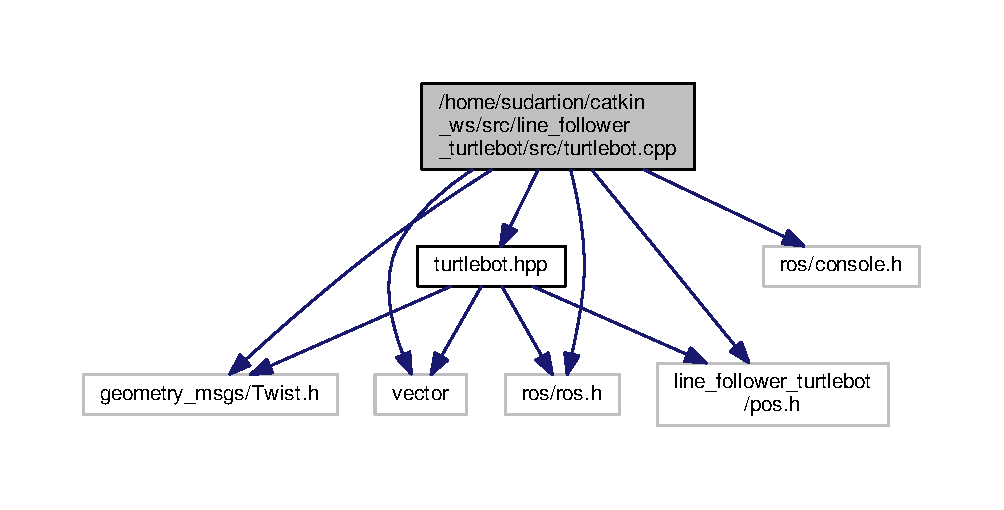
\includegraphics[width=350pt]{turtlebot_8cpp__incl}
\end{center}
\end{figure}


\subsection{Detailed Description}
Functions definitions for turtlebot class. 

M\+IT License Copyright (c) 2017 Sudarshan Raghunathan Permission is hereby granted, free of charge, to any person obtaining a copy of this software and associated documentation files (the \char`\"{}\+Software\char`\"{}), to deal in the Software without restriction, including without limitation the rights to use, copy, modify, merge, publish, distribute, sublicense, and/or sell copies of the Software, and to permit persons to whom the Software is furnished to do so, subject to the following conditions\+: The above copyright notice and this permission notice shall be included in all copies or substantial portions of the Software. T\+HE S\+O\+F\+T\+W\+A\+RE IS P\+R\+O\+V\+I\+D\+ED \char`\"{}\+A\+S I\+S\char`\"{}, W\+I\+T\+H\+O\+UT W\+A\+R\+R\+A\+N\+TY OF A\+NY K\+I\+ND, E\+X\+P\+R\+E\+SS OR I\+M\+P\+L\+I\+ED, I\+N\+C\+L\+U\+D\+I\+NG B\+UT N\+OT L\+I\+M\+I\+T\+ED TO T\+HE W\+A\+R\+R\+A\+N\+T\+I\+ES OF M\+E\+R\+C\+H\+A\+N\+T\+A\+B\+I\+L\+I\+TY, F\+I\+T\+N\+E\+SS F\+OR A P\+A\+R\+T\+I\+C\+U\+L\+AR P\+U\+R\+P\+O\+SE A\+ND N\+O\+N\+I\+N\+F\+R\+I\+N\+G\+E\+M\+E\+NT. IN NO E\+V\+E\+NT S\+H\+A\+LL T\+HE A\+U\+T\+H\+O\+RS OR C\+O\+P\+Y\+R\+I\+G\+HT H\+O\+L\+D\+E\+RS BE L\+I\+A\+B\+LE F\+OR A\+NY C\+L\+A\+IM, D\+A\+M\+A\+G\+ES OR O\+T\+H\+ER L\+I\+A\+B\+I\+L\+I\+TY, W\+H\+E\+T\+H\+ER IN AN A\+C\+T\+I\+ON OF C\+O\+N\+T\+R\+A\+CT, T\+O\+RT OR O\+T\+H\+E\+R\+W\+I\+SE, A\+R\+I\+S\+I\+NG F\+R\+OM, O\+UT OF OR IN C\+O\+N\+N\+E\+C\+T\+I\+ON W\+I\+TH T\+HE S\+O\+F\+T\+W\+A\+RE OR T\+HE U\+SE OR O\+T\+H\+ER D\+E\+A\+L\+I\+N\+GS IN T\+HE S\+O\+F\+T\+W\+A\+RE.

\begin{DoxyCopyright}{Copyright}
Copyright 2017 Sudarshan Raghunathan
\end{DoxyCopyright}
\begin{DoxyAuthor}{Author}
Sudarshan Raghunathan 
\end{DoxyAuthor}

\hypertarget{test__detect_8cpp}{}\section{/home/sudartion/catkin\+\_\+ws/src/line\+\_\+follower\+\_\+turtlebot/test/test\+\_\+detect.cpp File Reference}
\label{test__detect_8cpp}\index{/home/sudartion/catkin\+\_\+ws/src/line\+\_\+follower\+\_\+turtlebot/test/test\+\_\+detect.\+cpp@{/home/sudartion/catkin\+\_\+ws/src/line\+\_\+follower\+\_\+turtlebot/test/test\+\_\+detect.\+cpp}}


Unit Test for all the functions in the detection class.  


{\ttfamily \#include $<$cv\+\_\+bridge/cv\+\_\+bridge.\+h$>$}\\*
{\ttfamily \#include $<$gtest/gtest.\+h$>$}\\*
{\ttfamily \#include $<$opencv2/highgui/highgui.\+hpp$>$}\\*
{\ttfamily \#include \char`\"{}ros/ros.\+h\char`\"{}}\\*
{\ttfamily \#include \char`\"{}opencv2/opencv.\+hpp\char`\"{}}\\*
{\ttfamily \#include \char`\"{}linedetect.\+hpp\char`\"{}}\\*
{\ttfamily \#include \char`\"{}line\+\_\+follower\+\_\+turtlebot/pos.\+h\char`\"{}}\\*
Include dependency graph for test\+\_\+detect.\+cpp\+:\nopagebreak
\begin{figure}[H]
\begin{center}
\leavevmode
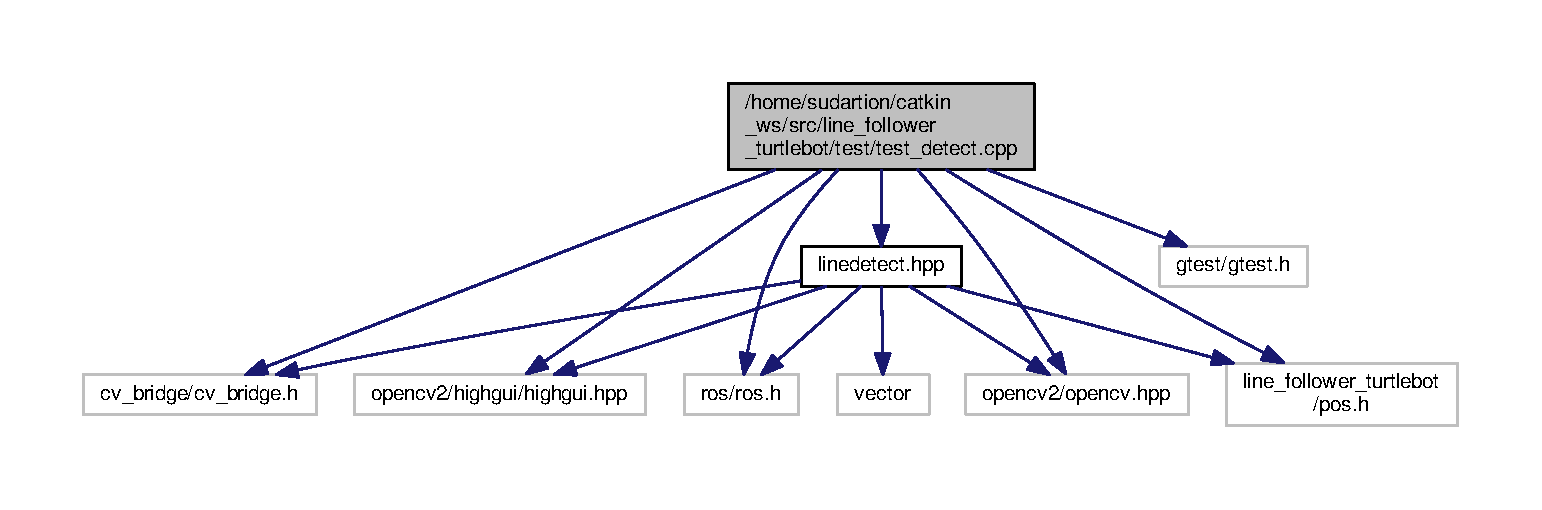
\includegraphics[width=350pt]{test__detect_8cpp__incl}
\end{center}
\end{figure}
\subsection*{Functions}
\begin{DoxyCompactItemize}
\item 
int \hyperlink{test__detect_8cpp_aab996c40807242ca60f59b84fab5b39f}{turn\+\_\+left} ()
\begin{DoxyCompactList}\small\item\em Testing if detection works accurately and publishes left accurately. \end{DoxyCompactList}\item 
int \hyperlink{test__detect_8cpp_adafa16f901d157cb8393ac413808231a}{drive\+\_\+straight} ()
\begin{DoxyCompactList}\small\item\em Testing if detection works accurately and publishes straight accurately. \end{DoxyCompactList}\item 
int \hyperlink{test__detect_8cpp_acc5172ce4388a6d7fddb6bc93fb31b3f}{turn\+\_\+right} ()
\begin{DoxyCompactList}\small\item\em Testing if detection works accurately and publishes right accurately. \end{DoxyCompactList}\item 
int \hyperlink{test__detect_8cpp_ae51416af540512a3ba419ad44754360e}{stop} ()
\begin{DoxyCompactList}\small\item\em Testing if detection works accurately and publishes stop accurately. \end{DoxyCompactList}\item 
bool \hyperlink{test__detect_8cpp_ae47c8c035bbf706e10084b39bcf91eeb}{gauss} ()
\begin{DoxyCompactList}\small\item\em Testing if gaussian filtering functions properly. \end{DoxyCompactList}\item 
\hyperlink{test__detect_8cpp_a39dfd2a96a80546eba2e777cb13c88e8}{T\+E\+ST} (Test\+Directions, Teststraight)\hypertarget{test__detect_8cpp_a39dfd2a96a80546eba2e777cb13c88e8}{}\label{test__detect_8cpp_a39dfd2a96a80546eba2e777cb13c88e8}

\begin{DoxyCompactList}\small\item\em Testing if direction published is straight. \end{DoxyCompactList}\item 
\hyperlink{test__detect_8cpp_ad5605f855f69cece94263f8f1cca0954}{T\+E\+ST} (Test\+Directions, Testleft)\hypertarget{test__detect_8cpp_ad5605f855f69cece94263f8f1cca0954}{}\label{test__detect_8cpp_ad5605f855f69cece94263f8f1cca0954}

\begin{DoxyCompactList}\small\item\em Testing if direction published is left. \end{DoxyCompactList}\item 
\hyperlink{test__detect_8cpp_aaf48f4ae6bba9d5d30ca112624980e98}{T\+E\+ST} (Test\+Directions, Testright)\hypertarget{test__detect_8cpp_aaf48f4ae6bba9d5d30ca112624980e98}{}\label{test__detect_8cpp_aaf48f4ae6bba9d5d30ca112624980e98}

\begin{DoxyCompactList}\small\item\em Testing if direction published is right. \end{DoxyCompactList}\item 
\hyperlink{test__detect_8cpp_a8e61dbed625cc9a28c0ead0cd032a19c}{T\+E\+ST} (Test\+Directions, Teststop)\hypertarget{test__detect_8cpp_a8e61dbed625cc9a28c0ead0cd032a19c}{}\label{test__detect_8cpp_a8e61dbed625cc9a28c0ead0cd032a19c}

\begin{DoxyCompactList}\small\item\em Testing if stop command is published. \end{DoxyCompactList}\item 
\hyperlink{test__detect_8cpp_a06f780fde9cb11239a23e9fdd89b879d}{T\+E\+ST} (Test\+Det\+Func, Test\+Gauss)\hypertarget{test__detect_8cpp_a06f780fde9cb11239a23e9fdd89b879d}{}\label{test__detect_8cpp_a06f780fde9cb11239a23e9fdd89b879d}

\begin{DoxyCompactList}\small\item\em Testing if Gaussian filter is applied to image properly. \end{DoxyCompactList}\item 
int \hyperlink{test__detect_8cpp_a3c04138a5bfe5d72780bb7e82a18e627}{main} (int argc, char $\ast$$\ast$argv)
\begin{DoxyCompactList}\small\item\em Function to run all the tests for the detection node. \end{DoxyCompactList}\end{DoxyCompactItemize}


\subsection{Detailed Description}
Unit Test for all the functions in the detection class. 

M\+IT License Copyright (c) 2017 Sudarshan Raghunathan Permission is hereby granted, free of charge, to any person obtaining a copy of this software and associated documentation files (the \char`\"{}\+Software\char`\"{}), to deal in the Software without restriction, including without limitation the rights to use, copy, modify, merge, publish, distribute, sublicense, and/or sell copies of the Software, and to permit persons to whom the Software is furnished to do so, subject to the following conditions\+: The above copyright notice and this permission notice shall be included in all copies or substantial portions of the Software. T\+HE S\+O\+F\+T\+W\+A\+RE IS P\+R\+O\+V\+I\+D\+ED \char`\"{}\+A\+S I\+S\char`\"{}, W\+I\+T\+H\+O\+UT W\+A\+R\+R\+A\+N\+TY OF A\+NY K\+I\+ND, E\+X\+P\+R\+E\+SS OR I\+M\+P\+L\+I\+ED, I\+N\+C\+L\+U\+D\+I\+NG B\+UT N\+OT L\+I\+M\+I\+T\+ED TO T\+HE W\+A\+R\+R\+A\+N\+T\+I\+ES OF M\+E\+R\+C\+H\+A\+N\+T\+A\+B\+I\+L\+I\+TY, F\+I\+T\+N\+E\+SS F\+OR A P\+A\+R\+T\+I\+C\+U\+L\+AR P\+U\+R\+P\+O\+SE A\+ND N\+O\+N\+I\+N\+F\+R\+I\+N\+G\+E\+M\+E\+NT. IN NO E\+V\+E\+NT S\+H\+A\+LL T\+HE A\+U\+T\+H\+O\+RS OR C\+O\+P\+Y\+R\+I\+G\+HT H\+O\+L\+D\+E\+RS BE L\+I\+A\+B\+LE F\+OR A\+NY C\+L\+A\+IM, D\+A\+M\+A\+G\+ES OR O\+T\+H\+ER L\+I\+A\+B\+I\+L\+I\+TY, W\+H\+E\+T\+H\+ER IN AN A\+C\+T\+I\+ON OF C\+O\+N\+T\+R\+A\+CT, T\+O\+RT OR O\+T\+H\+E\+R\+W\+I\+SE, A\+R\+I\+S\+I\+NG F\+R\+OM, O\+UT OF OR IN C\+O\+N\+N\+E\+C\+T\+I\+ON W\+I\+TH T\+HE S\+O\+F\+T\+W\+A\+RE OR T\+HE U\+SE OR O\+T\+H\+ER D\+E\+A\+L\+I\+N\+GS IN T\+HE S\+O\+F\+T\+W\+A\+RE.

\begin{DoxyCopyright}{Copyright}
Copyright 2017 Sudarshan Raghunathan
\end{DoxyCopyright}
\begin{DoxyAuthor}{Author}
Sudarshan Raghunathan 
\end{DoxyAuthor}


\subsection{Function Documentation}
\index{test\+\_\+detect.\+cpp@{test\+\_\+detect.\+cpp}!drive\+\_\+straight@{drive\+\_\+straight}}
\index{drive\+\_\+straight@{drive\+\_\+straight}!test\+\_\+detect.\+cpp@{test\+\_\+detect.\+cpp}}
\subsubsection[{\texorpdfstring{drive\+\_\+straight()}{drive_straight()}}]{\setlength{\rightskip}{0pt plus 5cm}int drive\+\_\+straight (
\begin{DoxyParamCaption}
{}
\end{DoxyParamCaption}
)}\hypertarget{test__detect_8cpp_adafa16f901d157cb8393ac413808231a}{}\label{test__detect_8cpp_adafa16f901d157cb8393ac413808231a}


Testing if detection works accurately and publishes straight accurately. 

\begin{DoxyReturn}{Returns}
int dir which is the direction to move in 
\end{DoxyReturn}
\index{test\+\_\+detect.\+cpp@{test\+\_\+detect.\+cpp}!gauss@{gauss}}
\index{gauss@{gauss}!test\+\_\+detect.\+cpp@{test\+\_\+detect.\+cpp}}
\subsubsection[{\texorpdfstring{gauss()}{gauss()}}]{\setlength{\rightskip}{0pt plus 5cm}bool gauss (
\begin{DoxyParamCaption}
{}
\end{DoxyParamCaption}
)}\hypertarget{test__detect_8cpp_ae47c8c035bbf706e10084b39bcf91eeb}{}\label{test__detect_8cpp_ae47c8c035bbf706e10084b39bcf91eeb}


Testing if gaussian filtering functions properly. 

\begin{DoxyReturn}{Returns}
bool to test if function worked well 
\end{DoxyReturn}
\index{test\+\_\+detect.\+cpp@{test\+\_\+detect.\+cpp}!main@{main}}
\index{main@{main}!test\+\_\+detect.\+cpp@{test\+\_\+detect.\+cpp}}
\subsubsection[{\texorpdfstring{main(int argc, char $\ast$$\ast$argv)}{main(int argc, char **argv)}}]{\setlength{\rightskip}{0pt plus 5cm}int main (
\begin{DoxyParamCaption}
\item[{int}]{argc, }
\item[{char $\ast$$\ast$}]{argv}
\end{DoxyParamCaption}
)}\hypertarget{test__detect_8cpp_a3c04138a5bfe5d72780bb7e82a18e627}{}\label{test__detect_8cpp_a3c04138a5bfe5d72780bb7e82a18e627}


Function to run all the tests for the detection node. 


\begin{DoxyParams}{Parameters}
{\em argc} & is the number of arguments of the main function \\
\hline
{\em argv} & is the array of arugments \\
\hline
\end{DoxyParams}
\begin{DoxyReturn}{Returns}
result of the tests 
\end{DoxyReturn}
\index{test\+\_\+detect.\+cpp@{test\+\_\+detect.\+cpp}!stop@{stop}}
\index{stop@{stop}!test\+\_\+detect.\+cpp@{test\+\_\+detect.\+cpp}}
\subsubsection[{\texorpdfstring{stop()}{stop()}}]{\setlength{\rightskip}{0pt plus 5cm}int stop (
\begin{DoxyParamCaption}
{}
\end{DoxyParamCaption}
)}\hypertarget{test__detect_8cpp_ae51416af540512a3ba419ad44754360e}{}\label{test__detect_8cpp_ae51416af540512a3ba419ad44754360e}


Testing if detection works accurately and publishes stop accurately. 

\begin{DoxyReturn}{Returns}
int dir which is the direction to move in 
\end{DoxyReturn}
\index{test\+\_\+detect.\+cpp@{test\+\_\+detect.\+cpp}!turn\+\_\+left@{turn\+\_\+left}}
\index{turn\+\_\+left@{turn\+\_\+left}!test\+\_\+detect.\+cpp@{test\+\_\+detect.\+cpp}}
\subsubsection[{\texorpdfstring{turn\+\_\+left()}{turn_left()}}]{\setlength{\rightskip}{0pt plus 5cm}int turn\+\_\+left (
\begin{DoxyParamCaption}
{}
\end{DoxyParamCaption}
)}\hypertarget{test__detect_8cpp_aab996c40807242ca60f59b84fab5b39f}{}\label{test__detect_8cpp_aab996c40807242ca60f59b84fab5b39f}


Testing if detection works accurately and publishes left accurately. 

\begin{DoxyReturn}{Returns}
int dir which is the direction to move in 
\end{DoxyReturn}
\index{test\+\_\+detect.\+cpp@{test\+\_\+detect.\+cpp}!turn\+\_\+right@{turn\+\_\+right}}
\index{turn\+\_\+right@{turn\+\_\+right}!test\+\_\+detect.\+cpp@{test\+\_\+detect.\+cpp}}
\subsubsection[{\texorpdfstring{turn\+\_\+right()}{turn_right()}}]{\setlength{\rightskip}{0pt plus 5cm}int turn\+\_\+right (
\begin{DoxyParamCaption}
{}
\end{DoxyParamCaption}
)}\hypertarget{test__detect_8cpp_acc5172ce4388a6d7fddb6bc93fb31b3f}{}\label{test__detect_8cpp_acc5172ce4388a6d7fddb6bc93fb31b3f}


Testing if detection works accurately and publishes right accurately. 

\begin{DoxyReturn}{Returns}
int dir which is the direction to move in 
\end{DoxyReturn}

\hypertarget{test__navig_8cpp}{}\section{/home/sudartion/catkin\+\_\+ws/src/line\+\_\+follower\+\_\+turtlebot/test/test\+\_\+navig.cpp File Reference}
\label{test__navig_8cpp}\index{/home/sudartion/catkin\+\_\+ws/src/line\+\_\+follower\+\_\+turtlebot/test/test\+\_\+navig.\+cpp@{/home/sudartion/catkin\+\_\+ws/src/line\+\_\+follower\+\_\+turtlebot/test/test\+\_\+navig.\+cpp}}


Unit Test for all the functions in the turtlebot navigation class.  


{\ttfamily \#include $<$cstdlib$>$}\\*
{\ttfamily \#include $<$string$>$}\\*
{\ttfamily \#include $<$ros/package.\+h$>$}\\*
{\ttfamily \#include $<$sstream$>$}\\*
{\ttfamily \#include $<$opencv2/highgui/highgui.\+hpp$>$}\\*
{\ttfamily \#include $<$cv\+\_\+bridge/cv\+\_\+bridge.\+h$>$}\\*
{\ttfamily \#include $<$gtest/gtest.\+h$>$}\\*
{\ttfamily \#include $<$boost/thread.\+hpp$>$}\\*
{\ttfamily \#include \char`\"{}opencv2/opencv.\+hpp\char`\"{}}\\*
{\ttfamily \#include \char`\"{}ros/ros.\+h\char`\"{}}\\*
{\ttfamily \#include \char`\"{}ros/console.\+h\char`\"{}}\\*
{\ttfamily \#include \char`\"{}turtlebot.\+hpp\char`\"{}}\\*
{\ttfamily \#include \char`\"{}line\+\_\+follower\+\_\+turtlebot/pos.\+h\char`\"{}}\\*
Include dependency graph for test\+\_\+navig.\+cpp\+:\nopagebreak
\begin{figure}[H]
\begin{center}
\leavevmode
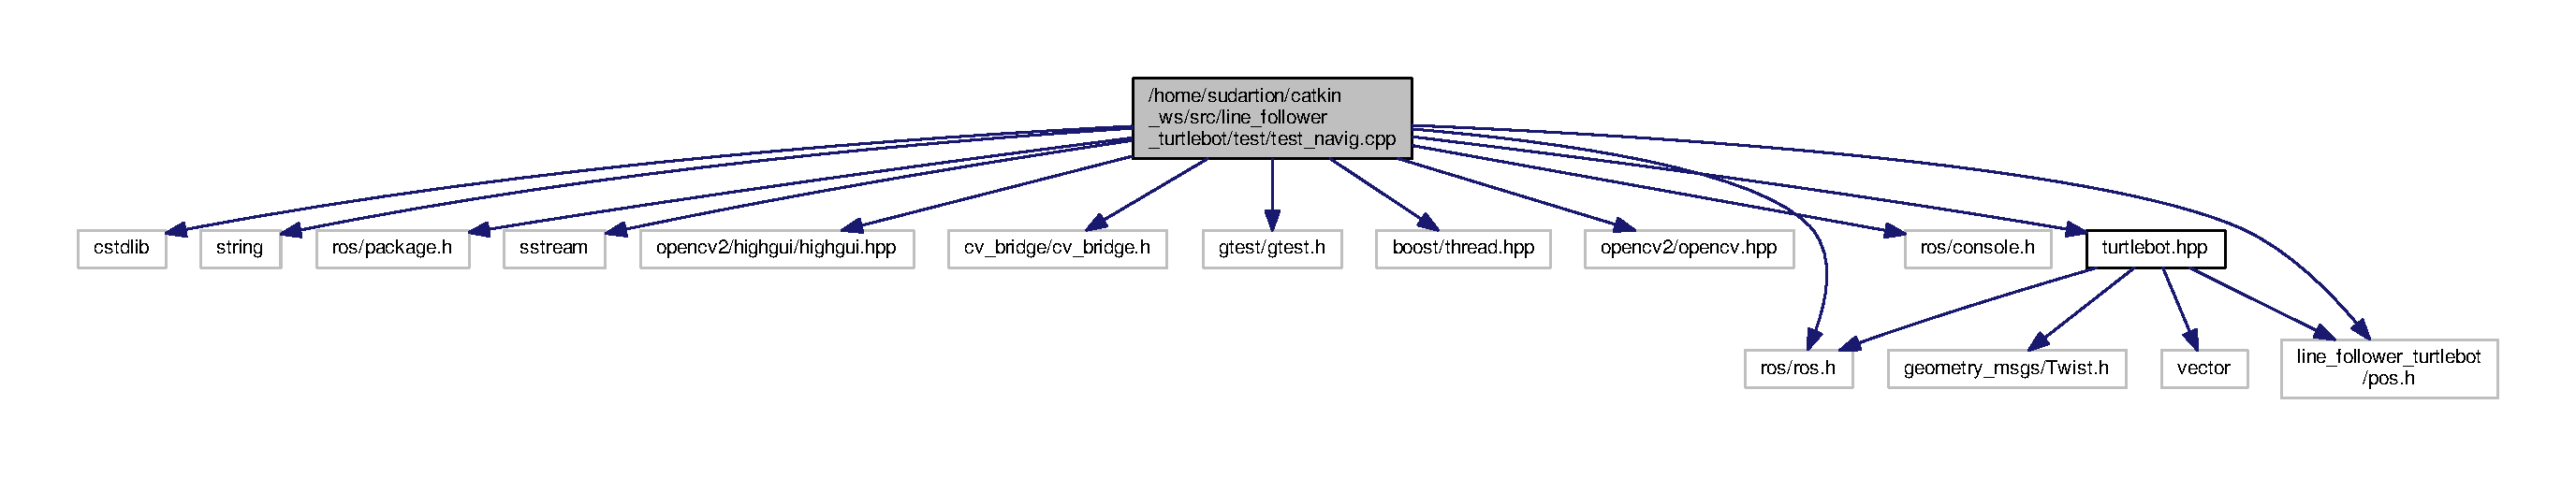
\includegraphics[width=350pt]{test__navig_8cpp__incl}
\end{center}
\end{figure}
\subsection*{Functions}
\begin{DoxyCompactItemize}
\item 
double \hyperlink{test__navig_8cpp_a3298bf3dc9e8eeece37641ff08ff6dcb}{ang\+\_\+vel} (int direction)
\begin{DoxyCompactList}\small\item\em Testing if detection works accurately and publishes straight accurately. \end{DoxyCompactList}\item 
double \hyperlink{test__navig_8cpp_ab648b8839cb39d17588b2aaf43bdf1d2}{linear\+\_\+vel} (int direction)
\begin{DoxyCompactList}\small\item\em Testing if detection works accurately and publishes straight accurately. \end{DoxyCompactList}\item 
void \hyperlink{test__navig_8cpp_abee919b3b96d4d58ae9a6c4952b67c22}{process\+Thread} (void)\hypertarget{test__navig_8cpp_abee919b3b96d4d58ae9a6c4952b67c22}{}\label{test__navig_8cpp_abee919b3b96d4d58ae9a6c4952b67c22}

\begin{DoxyCompactList}\small\item\em Function to spin the callbacks at a specific rate. \end{DoxyCompactList}\item 
\hyperlink{test__navig_8cpp_a16f601553263f11e30380d1c429c2b98}{T\+E\+ST} (Test\+R\+OS, Test\+Pub\+Sub)\hypertarget{test__navig_8cpp_a16f601553263f11e30380d1c429c2b98}{}\label{test__navig_8cpp_a16f601553263f11e30380d1c429c2b98}

\begin{DoxyCompactList}\small\item\em Testing if message subscriber is working properly. \end{DoxyCompactList}\item 
\hyperlink{test__navig_8cpp_adabbc7231644472f24d8056fd42b2d5a}{T\+E\+ST} (Test\+Velocity, Teststraight\+\_\+vel)\hypertarget{test__navig_8cpp_adabbc7231644472f24d8056fd42b2d5a}{}\label{test__navig_8cpp_adabbc7231644472f24d8056fd42b2d5a}

\begin{DoxyCompactList}\small\item\em Testing if velocity published is for moving straight. \end{DoxyCompactList}\item 
\hyperlink{test__navig_8cpp_a6246853d1fb891135e2cfc3591b1d064}{T\+E\+ST} (Test\+Directions, Testleft\+\_\+vel)\hypertarget{test__navig_8cpp_a6246853d1fb891135e2cfc3591b1d064}{}\label{test__navig_8cpp_a6246853d1fb891135e2cfc3591b1d064}

\begin{DoxyCompactList}\small\item\em Testing if velocity published is for turning left. \end{DoxyCompactList}\item 
\hyperlink{test__navig_8cpp_ae8fdc3f364b5ed04b991184ea8aacae0}{T\+E\+ST} (Test\+Directions, Testright\+\_\+vel)\hypertarget{test__navig_8cpp_ae8fdc3f364b5ed04b991184ea8aacae0}{}\label{test__navig_8cpp_ae8fdc3f364b5ed04b991184ea8aacae0}

\begin{DoxyCompactList}\small\item\em Testing if velocity published is for turning right. \end{DoxyCompactList}\item 
\hyperlink{test__navig_8cpp_af6f3ba161b8fc49e30c037b43c4b76ec}{T\+E\+ST} (Test\+Directions, Teststop\+\_\+vel)\hypertarget{test__navig_8cpp_af6f3ba161b8fc49e30c037b43c4b76ec}{}\label{test__navig_8cpp_af6f3ba161b8fc49e30c037b43c4b76ec}

\begin{DoxyCompactList}\small\item\em Testing if velocity published is for stopping. \end{DoxyCompactList}\item 
int \hyperlink{test__navig_8cpp_a3c04138a5bfe5d72780bb7e82a18e627}{main} (int argc, char $\ast$$\ast$argv)
\begin{DoxyCompactList}\small\item\em Function to run all the tests for the navigation node. \end{DoxyCompactList}\end{DoxyCompactItemize}


\subsection{Detailed Description}
Unit Test for all the functions in the turtlebot navigation class. 

M\+IT License Copyright (c) 2017 Sudarshan Raghunathan Permission is hereby granted, free of charge, to any person obtaining a copy of this software and associated documentation files (the \char`\"{}\+Software\char`\"{}), to deal in the Software without restriction, including without limitation the rights to use, copy, modify, merge, publish, distribute, sublicense, and/or sell copies of the Software, and to permit persons to whom the Software is furnished to do so, subject to the following conditions\+: The above copyright notice and this permission notice shall be included in all copies or substantial portions of the Software. T\+HE S\+O\+F\+T\+W\+A\+RE IS P\+R\+O\+V\+I\+D\+ED \char`\"{}\+A\+S I\+S\char`\"{}, W\+I\+T\+H\+O\+UT W\+A\+R\+R\+A\+N\+TY OF A\+NY K\+I\+ND, E\+X\+P\+R\+E\+SS OR I\+M\+P\+L\+I\+ED, I\+N\+C\+L\+U\+D\+I\+NG B\+UT N\+OT L\+I\+M\+I\+T\+ED TO T\+HE W\+A\+R\+R\+A\+N\+T\+I\+ES OF M\+E\+R\+C\+H\+A\+N\+T\+A\+B\+I\+L\+I\+TY, F\+I\+T\+N\+E\+SS F\+OR A P\+A\+R\+T\+I\+C\+U\+L\+AR P\+U\+R\+P\+O\+SE A\+ND N\+O\+N\+I\+N\+F\+R\+I\+N\+G\+E\+M\+E\+NT. IN NO E\+V\+E\+NT S\+H\+A\+LL T\+HE A\+U\+T\+H\+O\+RS OR C\+O\+P\+Y\+R\+I\+G\+HT H\+O\+L\+D\+E\+RS BE L\+I\+A\+B\+LE F\+OR A\+NY C\+L\+A\+IM, D\+A\+M\+A\+G\+ES OR O\+T\+H\+ER L\+I\+A\+B\+I\+L\+I\+TY, W\+H\+E\+T\+H\+ER IN AN A\+C\+T\+I\+ON OF C\+O\+N\+T\+R\+A\+CT, T\+O\+RT OR O\+T\+H\+E\+R\+W\+I\+SE, A\+R\+I\+S\+I\+NG F\+R\+OM, O\+UT OF OR IN C\+O\+N\+N\+E\+C\+T\+I\+ON W\+I\+TH T\+HE S\+O\+F\+T\+W\+A\+RE OR T\+HE U\+SE OR O\+T\+H\+ER D\+E\+A\+L\+I\+N\+GS IN T\+HE S\+O\+F\+T\+W\+A\+RE.

\begin{DoxyCopyright}{Copyright}
Copyright 2017 Sudarshan Raghunathan
\end{DoxyCopyright}
\begin{DoxyAuthor}{Author}
Sudarshan Raghunathan 
\end{DoxyAuthor}


\subsection{Function Documentation}
\index{test\+\_\+navig.\+cpp@{test\+\_\+navig.\+cpp}!ang\+\_\+vel@{ang\+\_\+vel}}
\index{ang\+\_\+vel@{ang\+\_\+vel}!test\+\_\+navig.\+cpp@{test\+\_\+navig.\+cpp}}
\subsubsection[{\texorpdfstring{ang\+\_\+vel(int direction)}{ang_vel(int direction)}}]{\setlength{\rightskip}{0pt plus 5cm}double ang\+\_\+vel (
\begin{DoxyParamCaption}
\item[{int}]{direction}
\end{DoxyParamCaption}
)}\hypertarget{test__navig_8cpp_a3298bf3dc9e8eeece37641ff08ff6dcb}{}\label{test__navig_8cpp_a3298bf3dc9e8eeece37641ff08ff6dcb}


Testing if detection works accurately and publishes straight accurately. 

\begin{DoxyReturn}{Returns}
int dir which is the direction to move in 
\end{DoxyReturn}
\index{test\+\_\+navig.\+cpp@{test\+\_\+navig.\+cpp}!linear\+\_\+vel@{linear\+\_\+vel}}
\index{linear\+\_\+vel@{linear\+\_\+vel}!test\+\_\+navig.\+cpp@{test\+\_\+navig.\+cpp}}
\subsubsection[{\texorpdfstring{linear\+\_\+vel(int direction)}{linear_vel(int direction)}}]{\setlength{\rightskip}{0pt plus 5cm}double linear\+\_\+vel (
\begin{DoxyParamCaption}
\item[{int}]{direction}
\end{DoxyParamCaption}
)}\hypertarget{test__navig_8cpp_ab648b8839cb39d17588b2aaf43bdf1d2}{}\label{test__navig_8cpp_ab648b8839cb39d17588b2aaf43bdf1d2}


Testing if detection works accurately and publishes straight accurately. 

\begin{DoxyReturn}{Returns}
int dir which is the direction to move in 
\end{DoxyReturn}
\index{test\+\_\+navig.\+cpp@{test\+\_\+navig.\+cpp}!main@{main}}
\index{main@{main}!test\+\_\+navig.\+cpp@{test\+\_\+navig.\+cpp}}
\subsubsection[{\texorpdfstring{main(int argc, char $\ast$$\ast$argv)}{main(int argc, char **argv)}}]{\setlength{\rightskip}{0pt plus 5cm}int main (
\begin{DoxyParamCaption}
\item[{int}]{argc, }
\item[{char $\ast$$\ast$}]{argv}
\end{DoxyParamCaption}
)}\hypertarget{test__navig_8cpp_a3c04138a5bfe5d72780bb7e82a18e627}{}\label{test__navig_8cpp_a3c04138a5bfe5d72780bb7e82a18e627}


Function to run all the tests for the navigation node. 


\begin{DoxyParams}{Parameters}
{\em argc} & is the number of arguments of the main function \\
\hline
{\em argv} & is the array of arugments \\
\hline
\end{DoxyParams}
\begin{DoxyReturn}{Returns}
result of the tests 
\end{DoxyReturn}

%--- End generated contents ---

% Index
\backmatter
\newpage
\phantomsection
\clearemptydoublepage
\addcontentsline{toc}{chapter}{Index}
\printindex

\end{document}
